\documentclass[conference]{IEEEtran}
\usepackage[T1]{fontenc}
\usepackage{lmodern}
\usepackage[draft]{hyperref}
\usepackage{url}
\usepackage{cite} % Multiple citations in one~\cite command
\usepackage{pgfplotstable}
\usepackage{array} % Required for pgfplotstable dec sep align
\pgfplotsset{compat=1.12}
\usepackage{booktabs}
\usepackage{todonotes}
\usepackage{listings}

%\newcommand{\todob}[1]{\todo[inline,color=green!40]{#1}}

\usepackage{enumitem}
\setlist{parsep=0pt, listparindent=0.5cm}
\pdfminorversion=7

\begin{document}
\title{A Comparison of Parallel Graph Processing Implementations}
\author{
	\IEEEauthorblockN{Samuel D. Pollard}
	\IEEEauthorblockA{Computer and Information Science\\
		University of Oregon \\
		Eugene, OR 97403\\
		Email: spollard@cs.uoregon.edu}
	\and
	\IEEEauthorblockN{Boyana Norris}
	\IEEEauthorblockA{Computer and Information Science\\
		University of Oregon \\
		Eugene, OR 97403\\
		Email: norris@cs.uoregon.edu}
}
\maketitle

\begin{abstract}
The rapidly growing number of large network analysis problems has led to the emergence of many parallel and distributed graph processing systems---one survey in 2014 identified over 80. Determining the best approach for a given problem is infeasible for most developers. We present an approach and associated software for analyzing the performance and scalability of parallel, open-source graph libraries. We demonstrate our approach on five graph processing packages: GraphMat, Graph500, Graph Algorithm Platform Benchmark Suite, GraphBIG, and PowerGraph using synthetic and real-world datasets. We examine previously overlooked aspects of parallel graph processing performance such as phases of execution and energy usage for three algorithms: breadth first search, single source shortest paths, and PageRank.
\end{abstract}

\section{Extended Abstract}

\subsection{Motivation}
Any user wishing to perform graph analytics faces the daunting task of selecting which software package to use given a problem. Installing, satisfying dependencies, and determining which algorithms are supported is nontrivial. Input file formats, and stopping criteria vary across packages.

\subsection{Architectural Overview}
Our framework, easy-parallel-graph-\textasteriskcentered, comprises Bash shell scripts which automate each step of the experiment. Our framework breaks the process of characterizing performance into five principal phases as follows.
\begin{enumerate}
	\item Installing modified, stable forks of each software package to ensure homogeneity.
	\item Given a synthetic graph size or a real-world graph file, generate the files necessary to run each software package.
	\item Given a graph and the number of threads, run each algorithm using each software package multiple times.
	\item Parse through the log files to compress the output into a CSV.
	\item Analyze the data using the provided R scripts to generate plots.
\end{enumerate}
The source code is freely available at \url{https://github.com/HPCL/easy-parallel-graph}.

%\begin{figure*}
%	\centering
%	% trim=left lower right upper
%	\includegraphics[width=0.8\linewidth, trim=0 8pt 0pt 8pt, clip]{graphics/overview.eps}
%	\caption{Overview of \emph{easy-parallel-graph-\textasteriskcentered}. Each cyan box corresponds to a single shell script in the package while the green ellipses correspond to generated files.}
%	\label{fig:epg-overview}
%\end{figure*}

\subsection{Algorithms and Packges}
We provide analysis for three algorithms and five packages, though not all packages implement all algorithms. The algorithms are Breadth First Search (BFS), Single Source Shortest Paths (SSSP), and PageRank. The packages are listed below:

\begin{enumerate}
	\item The Graph500~\cite{Murphy:2010:Graph500} consists of a specification and reference implementation of BFS.
	\item The Graph Algorithm Platform (GAP) Benchmark Suite~\cite{Beamer:2015:GAPBench}, a set of reference implementations for shared memory graph processing. GAP implements all three algorithms.
	\item GraphBIG~\cite{Nai:2015:Graphbig} benchmark suite, all three algorithms.
	\item GraphMat~\cite{Sundaram:2015:GraphMat}, a library and programming model, all three algorithms.
	\item PowerGraph~\cite{Gonzalez:2012:Powergraph}, a library for distributed and shared memory graph-parallel computation. Powergraph provides SSSP and PageRank reference implementations.
\end{enumerate}

\subsection{Related Work}\label{sec:relatedwork}
Graphalytics~\cite{Capota:2015:Graphalytics} is the most prominent benchmark suite presented and is still active. Other benchmark suites which to the best of our knowledge do not have associated publications are GraphBench\footnote{\url{https://github.com/uwsampa/graphbench}} and Graph Package Testing\footnote{\url{ https://github.com/robmccoll/graphdb-testing}}. Additionally, each graph processing package typically presents its own performance analysis.

\subsection{Datasets}
Our framework supports synthetic datasets consisting of Kronecker Graphs~\cite{Leskovec:2010:Kronecker}, a generalization of the RMAT graphs and are used in the Graph500.

Additionally, any dataset in the format of the Stanford Network Analysis Project~\cite{snapnets} (SNAP) may be used\footnote{This format is one edge per line with \# as comment lines.}. For our examples we use the Dota-League dataset~\cite{Guo:2012:GTA} and the cit-Patents dataset~\cite{snap-cit-patents}.

Each graph is made undirected and unweighted, then converted to the formats necessary for each implementations

\subsection{Results}

\begin{figure}
	\centering
	\begin{minipage}{0.7\linewidth}
		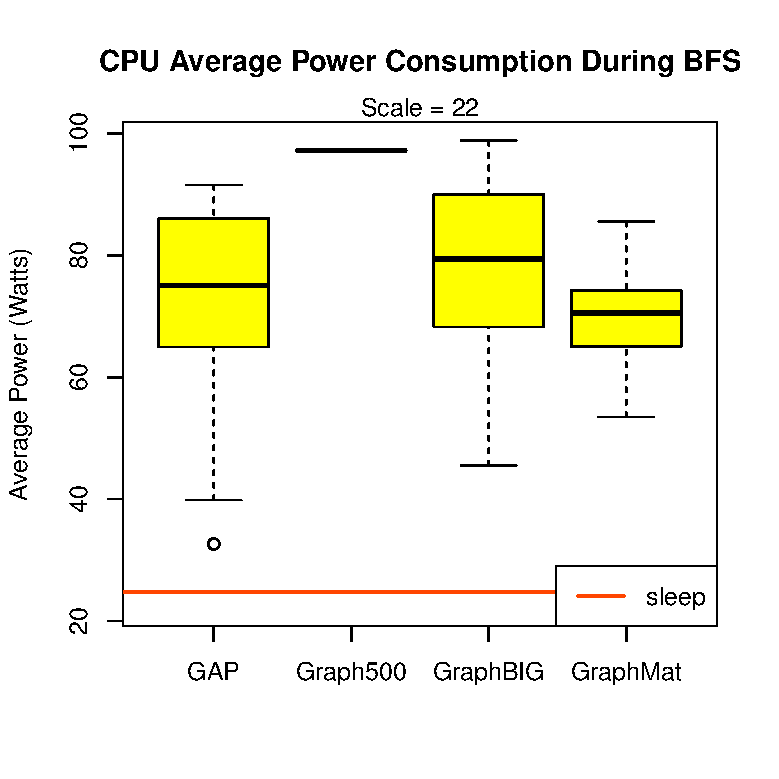
\includegraphics[width=\linewidth, trim=0 40pt 18pt 24pt, clip]{graphics/bfs_cpu_power.pdf}
	\end{minipage}
	\caption{We plot CPU Power Consumption for each of the 32 roots. Since Graph500 runs multiple roots per execution, we only get a single data point. The baseline monitors power consumption during the execution of the C \texttt{unistd} function \texttt{sleep(10)} (ten seconds).}
	\label{fig:power}
\end{figure}

We use the Performance Application Programming Interface (PAPI)~\cite{Browne:2000:PAPI} to access Intel's Running Average Power Limit (RAPL), which provides a set of hardware counters for measuring energy usage. Results from this are shown in Fig.~\ref{fig:power}.

\begin{figure}[htb]
	\centering
		% trim=left lower right upper
		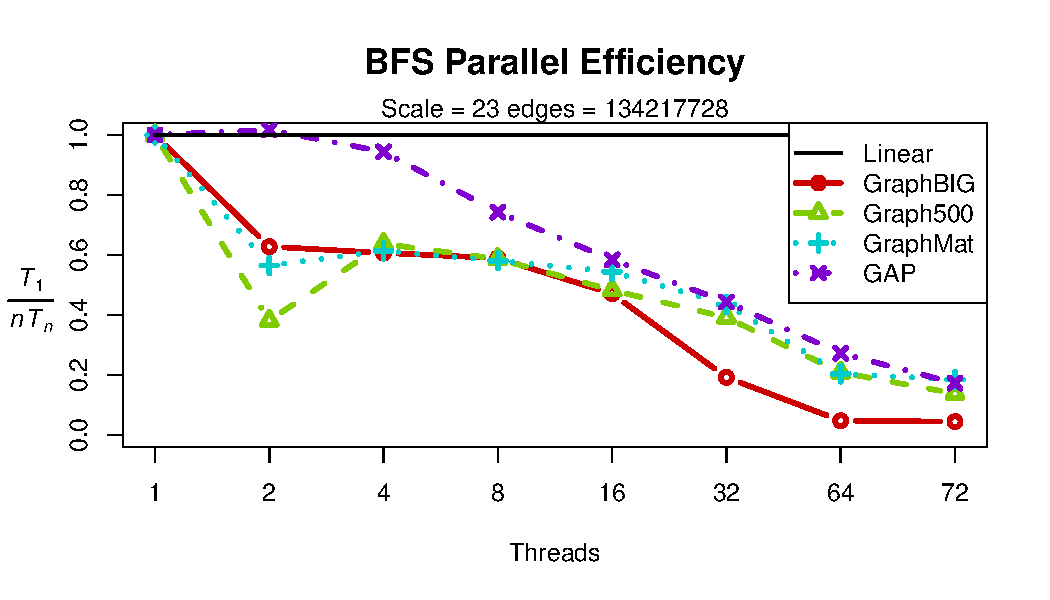
\includegraphics[width=0.95\linewidth, trim=0 18pt 24pt 18pt, clip]{graphics/bfs_ss23.pdf}
	\caption{Parallel efficiency for a scale-23 graph. $T_1$ is the serial time, $n$ is the number of threads, and $T_n$ is the time with $n$ threads.}
	\label{fig:bfs-efficiency}
\end{figure}
Figure~\ref{fig:bfs-efficiency} shows the parallel efficiency, $T_1 / (nT_n)$ for different implementations of BFS. Ideal efficiency is defined as $T_n = T_1/n$ and is the horizontal line near the top of Fig.~\ref{fig:bfs-efficiency}.

\begin{figure}
	\centering
	% trim=left lower right upper
	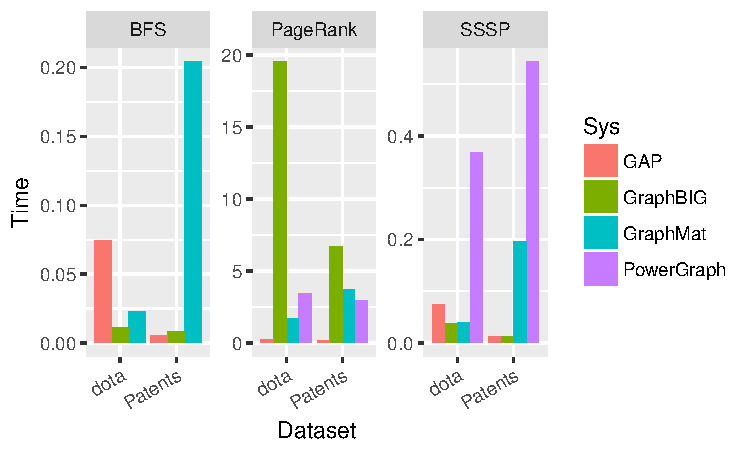
\includegraphics[width=0.95\linewidth, trim=0 18pt 6pt 6pt, clip]{graphics/compare-realworld.pdf}
	\caption{Real world experiments using \emph{easy-parallel-graph-\textasteriskcentered} averaged across 32 runs.}
	\label{fig:epg-realworld}
\end{figure}

Fig.~\ref{fig:epg-realworld} shows results for real-world experiments.

\subsection{Conclusion and Future Work}
A comparison of implementations requires tedious engineering effort. The newest framework, GAP, is the best performing framework in most cases.

Future improvements will add more algorithms and packages; support for triangle counting and Galois \cite{Nguyen:2013:Galois} is nearly complete.

Searching for optimal parameters for SSSP ($\Delta$-stepping) and BFS (direction-optimizing parameters $\alpha$ and $\beta$) via search would also increase performance for graph package users.

\bibliographystyle{IEEEtranS}
\bibliography{../drp}
\end{document}
